\chapter{Multi-Player Concurrent Reachability Games}

In this chapter, we first describe the notion of non-deterministic multi-player concurrent reachability games and define the solution concept of \textit{k-resilient} Nash equilibrium in these games. We then develop mathematical tools (\textit{k-suspect coalitions} and \textit{k-repellor sets}) to characterize \textit{k-resilient} Nash equilibria in these games when only pure strategies are allowed. We then prove some properties associated with \textit{k-suspect coalitions} and \textit{k-repellor sets}. These properties are then used to develop the algorithm to check the existence of \textit{k-resilient} Nash equilibrium in finite non-deterministic multi-player concurrent reachability games when only pure strategies are allowed. The properties that we prove also contain all the necessary information to compute a \textit{k-resilient} Nash equilibrium if it exists.

\section{Preliminaries}

In this section, we recall the definitions of some basic terms from \cite{BBM-concur10,BBM-report}. These terms are used throughout the thesis.

\begin{definition}
\label{def:transitionsystem}
A transition system $S$ is defined as a 2-tuple, $S = (States, Edg)$ where:
\begin{itemize}
\item $States$ is a possibly uncountable set of states.
\item $Edg \subseteq States \times States$ is the set of transitions (edges).
\end{itemize}
\end{definition}

A finite transition system is a transition system in which the set of states ($States$) is finite.

Given a transition system $S$, following terms are defined with respect to $S$:
\begin{enumerate}
\item A path $\pi$ in $S$, is a non-empty sequence $(s_{i})_{0\leq i<n}$ (where $n \in \mathbb{N} \cup \lbrace +\infty \rbrace$) of states of $S$ such that $(s_{i}, s_{i+1}) \in Edg$ for every $i < n-1$.
\item The length of a path $\pi = (s_{i})_{0\leq i<n}$ is denoted by $\vert \pi \vert$. $\vert \pi \vert = n-1$.
\item The set of finite paths (or \textit{histories}) of $S$ is denoted by $Hist_{S}$.
\item The set of infinite paths (or \textit{plays}) of $S$ is denoted by $Play_{S}$.
\item The set of all the paths of $S$ is denoted by $Path_{S}$. $Path_{S} = Hist_{S} \cup Play_{S}$.
\item Given a path $\pi = (s_{i})_{0\leq i<n}$ and an integer $j < n$, the $j^{th}$ prefix of $\pi$ (denoted by $\pi_{\leq j}$) is the finite path $(s_{i})_{0\leq i<j+1}$.
\item If a path $\pi$ is a history (a finite path), the last state of $\pi$ is denoted by $last(\pi)$. $last(\pi) = s_{\vert \pi \vert}$.    
\end{enumerate}

\section{Multi-Player Concurrent Reachability Games}

In this section, we describe the notion of non-deterministic multi-player concurrent reachability games as defined in \cite{BBM-concur10,BBM-report}. We then describe the concept of strategies, strategy profiles and the solution concept of \textit{k-resilient} Nash equilibrium in these games.

\begin{definition}
\label{def:game}
A non-deterministic multi-player concurrent reachability game $G$ is defined as a 7-tuple, $G = (States, Edg, Agt, Act, Mov, Tab, \Omega)$ where:
\begin{itemize}
\item $(States, Edg)$ is a transition system.
\item $Agt$ is a finite set of players (agents).
\item $Act$ is a possibly uncountable set of actions.
\item $Mov: States \times Agt \rightarrow 2^{Act}\setminus \lbrace \emptyset \rbrace$ is a mapping that indicates the actions available to a given player in a given state.
\item $Tab: States \times Act^{Agt} \rightarrow 2^{Edg}\setminus \lbrace \emptyset \rbrace$ is a mapping that associates a given tuple of actions of players in a given state to the resulting set of transitions. It is required that if $(s', s'') \in Tab(s, (m_{A})_{A\in Agt})$, then $s' = s$.
\item $\Omega : Agt \rightarrow 2^{States}$ is a mapping that assigns to each agent, a set of states, which is the reachability objective of that agent (i.e., the agent wants to reach at least one of these states).
\end{itemize}
\end{definition}

In a game $G$, from some state $s$, each player $A$ selects one action $m_{A}$ from its set $Mov(s, A)$ of allowed actions. The tuple of actions $(m_{A})_{A\in Agt}$ thus formed is called a move and is written as $m_{Agt}$. This results in a set of transitions $Tab(s, (m_{A})_{A\in Agt})$ (or simply $Tab(s, m_{Agt})$). One of these transitions is applied (non-deterministically) which gives the next state of the game. In this way, the game continues to form a path $\pi$ in its underlying transition system.

We associate a payoff vector $v_{Agt} = (v_{A})_{A\in Agt}$ to every path $\pi$ in $G$. If a path $\pi$ visits $\Omega (A)$ (i.e, at least one state in $\pi$ belongs to the set $\Omega (A)$), then we let $v_{A}(\pi) = 1$, otherwise $v_{A}(\pi) = 0$ (where $v_{A}(\pi)$ is the payoff received by player $A$, when the path $\pi$ is taken in $G$).

As in \cite{BBM-concur10,BBM-report}, we use the notations $Hist_{G}$, $Play_{G}$ and $Path_{G}$ for the set of \textit{histories}, \textit{plays} and \textit{paths} respectively, in the underlying transition system of $G$. We also write $Hist_{G}(s)$, $Play_{G}(s)$ and $Path_{G}(s)$ for respective subsets of \textit{histories}, \textit{plays} and \textit{paths} starting in state $s$.

We now recall the definitions of \textit{strategy} and \textit{strategy profile} from \cite{BBM-concur10,BBM-report}.
 
\begin{definition}
\label{def:strategy}
In a game $G$, a strategy for a player $A \in Agt$ is a mapping $\sigma_{A}: Hist_{G} \rightarrow Act$ such that for every $\pi \in Hist_{G}$, $\sigma_{A}(\pi) \in Mov(last(\pi), A)$.
\end{definition}

Given a subset of agents (also called a \textit{coalition}) $P \subseteq Agt$, a strategy $\sigma_{P}$ for the coalition $P$ is a tuple of strategies, one for each player in $P$ ($\sigma_{P} = (\sigma_{A})_{A\in P}$).

\begin{definition}
In a game $G$, a strategy profile $\sigma_{Agt}$ is a tuple of strategies, one for each player in $Agt$ (i.e., a strategy profile is a strategy for the coalition $Agt$). $\sigma_{Agt} = (\sigma_{A})_{A\in Agt}$.
\end{definition}

With respect to the sets of strategies, following notations are used in this thesis:
\begin{itemize}
\item $Strat^{A}_{G}$: Set of all strategies for a player $A \in Agt$ in a game $G$.
\item $Strat^{P}_{G}$: Set of all strategies for a coalition $P \subseteq Agt$ in a game $G$.
\item $Strat^{Agt}_{G}$: Set of all strategy profiles in a game $G$.
\end{itemize}

\begin{remark}
We only consider pure strategies (non-randomized strategies) in this thesis.
\end{remark}

In a game $G$, for a coalition $P$ and a strategy $\sigma_{P}$ (for $P$), a path $\pi = (s_{i})_{0\leq i\leq \vert \pi \vert}$ is said to be compatible with the strategy $\sigma_{P}$, if, for every $j \leq \vert \pi \vert - 1$, there is a move $m_{Agt} = (m_{A})_{A\in Agt}$ such that:
\begin{itemize}
\item $m_{A} \in Mov(s_{j}, A)$ for every $A \in Agt$.
\item $m_{A} = \sigma_{A}(\pi_{\leq j})$ for every $A \in P$.
\item $(s_{j}, s_{j+1}) \in Tab(s_{j}, m_{Agt})$ 
\end{itemize}

In a game $G$, the paths that are compatible with a strategy $\sigma_{P}$ (of a coalition $P$) are also called \textit{outcomes} of the strategy $\sigma_{P}$. We use the notation $Out_{G}(\sigma_{P})$ to denote the set of outcomes of strategy $\sigma_{P}$. The set of finite outcomes of strategy $\sigma_{P}$ is denoted by $Out_{G}^{f}(\sigma_{P})$. The set of infinite outcomes of strategy $\sigma_{P}$ is denoted by $Out_{G}^{\infty}(\sigma_{P})$. $Out_{G}(\sigma_{P}) = Out_{G}^{f}(\sigma_{P}) \cup Out_{G}^{\infty}(\sigma_{P})$. We write $Out_{G}(s, \sigma_{P})$, $Out_{G}^{f}(s, \sigma_{P})$ and $Out_{G}^{\infty}(s, \sigma_{P})$ for the respective sets of outcomes, finite outcomes and infinite outcomes of strategy $\sigma_{P}$ starting in state $s$. These notations are as used in \cite{BBM-concur10,BBM-report}.

In a game $G$, given a move $m_{Agt}$ and an action $m'_{B}$ for some player $B$, we write $m_{Agt}[B \rightarrow m'_{B}]$ for the move $n_{Agt}$ with $n_{A} = m_{A}$ when $A \neq B$ and $n_{B} = m'_{B}$.

In a game $G$, given a move $m_{Agt}$ and an action tuple $m'_{P}$ for a coalition $P$ ($m'_{P} = (m'_{A})_{A\in P}$), we write $m_{Agt}[P \rightarrow m'_{P}]$ for the move $n_{Agt}$ with $n_{A} = m_{A}$ for every $A \notin P$ and $n_{A} = m'_{A}$ for every $A \in P$.

In a game $G$, given a strategy profile $\alpha_{Agt} \in Strat^{Agt}_{G}$ and a strategy $\alpha'_{B}$ for some player $B$ ($\alpha'_{B} \in Strat^{B}_{G}$), we write $\alpha_{Agt}[B \rightarrow \alpha'_{B}]$ for the strategy profile $\beta_{Agt}$ with $\beta_{A} = \alpha_{A}$ when $A \neq B$ and $\beta_{B} = \alpha'_{B}$.

In a game $G$, given a strategy profile $\alpha_{Agt} \in Strat^{Agt}_{G}$ and a strategy $\alpha'_{P}$ for a coalition $P$ ($\alpha'_{P} \in Strat^{P}_{G}$), we write $\alpha_{Agt}[P \rightarrow \alpha'_{P}]$ for the strategy profile $\beta_{Agt}$ with $\beta_{A} = \alpha_{A}$ for every $A \notin P$ and $\beta_{A} = \alpha'_{A}$ for every $A \in P$.

In a game $G$, let $k$ be a non-negative integer such that $k \leq \vert Agt \vert$ ($k$ is a non-negative integer less than or equal to the number of players in $G$). We use the notation $2^{Agt}_{k}$ to denote the set of all subsets of $Agt$ of size at most $k$.
\[2^{Agt}_{k} = \lbrace P \; \vert \; P \in 2^{Agt} \; and \; \vert P \vert \leq k \rbrace\] 

We now extend the definition of \textit{pseudo-Nash equilibrium} given in \cite{BBM-concur10,BBM-report} to \textit{k-resilient pseudo-Nash equilibrium}.

\begin{definition}
Given a non-deterministic concurrent reachability game $G$ and a state $s$ in $G$, a \textit{k-resilient} pseudo-Nash equilibrium (for some $k \leq \vert Agt \vert$) in $G$ from $s$ is a pair $(\sigma_{Agt}, \pi)$ where $\sigma_{Agt} \in Strat^{Agt}_{G}$ and $\pi \in Out_{G}(s, \sigma_{Agt})$, such that, for every $P \in 2^{Agt}_{k}$ and every $\sigma'_{P} \in Strat^{P}_{G}$, it holds:
\[\forall \pi' \in Out_{G}(s, \sigma_{Agt}[P \rightarrow \sigma'_{P}]). \; \forall B \in P. \; v_{B}(\pi') \leq v_{B}(\pi)\]

Such an outcome $\pi$ is called a \textit{k-optimal} play for the strategy profile $\sigma_{Agt}$.
\end{definition}

The payoff vector of a \textit{k-resilient} pseudo-Nash equilibrium $(\sigma_{Agt}, \pi)$ is a tuple $(v_{A}(\pi))_{A \in Agt}$ where $v_{A}(\pi) = 1$ if $\pi$ visits $\Omega (A)$ and $v_{A}(\pi) = 0$ otherwise.

In case of deterministic concurrent reachability games, there is only one outcome of a given strategy profile ($\pi$ is uniquely determined by $\sigma_{Agt}$) and hence \textit{k-resilient} pseudo-Nash equilibria coincide with real \textit{k-resilient} Nash equilibria as defined in \cite{Abraham-2006,Abraham-2008}: they are strategy profiles such that, if at most $k$ players deviate from their respective strategies, none of the deviating player can benefit.

In case of non-deterministic concurrent reachability games, a strategy profile $\sigma_{Agt}$ for a \textit{k-resilient} pseudo-Nash equilibrium may give rise to several outcomes. The choice of playing the \textit{k-optimal} play $\pi$ is then made cooperatively by all the players. Once a strategy profile is fixed, non-determinism is resolved by all the players by choosing one of the possible outcomes in such a way that if at most $k$ players deviate from their respective strategies or choice of outcome, none of the deviating player can benefit.

\begin{example}
Figure \ref{fig:concurrentgame} shows a three-player concurrent reachability game. There are nine states in the game (labelled $s_{0}$ to $s_{8}$). The three players are $A$, $B$ and $C$. The actions allowed to player $A$ in state $s_{0}$ are $a_{1}$ and $a_{2}$. The actions allowed to player $B$ in state $s_{0}$ are $b_{1}$ and $b_{2}$. The actions allowed to player $C$ in state $s_{0}$ are $c_{1}$ and $c_{2}$. Edges in the game are labelled with a move (tuple of actions) of players. When players play a move (select their respective actions), the transition that corresponds to the played move is applied. Edges (transitions) starting in states $s_{1}$ to $s_{8}$ are self loops and are not labelled with any move. The transitions that are not labelled with any move can be applied for every possible tuple of actions (move) of players. Some states are also labelled with names of players in brackets. If a player's name appears in brackets within a state label, it means that the reachability set of that player contains that state. Observe that $\Omega (A) = \lbrace s_{3}, s_{6}, s_{7}, s_{8} \rbrace$, $\Omega (B) = \lbrace s_{1}, s_{3}, s_{4} \rbrace$ and $\Omega (C) = \lbrace s_{3}, s_{6}, s_{7}, s_{8} \rbrace$.

From state $s_{0}$, there are five Nash equilibria:
\begin{enumerate}
\item The strategy profile with the move $(a_{1}, b_{1}, c_{1})$ in state $s_{0}$ is a \textit{1-resilient} Nash equilibrium (or simply a Nash equilibrium).
\item The strategy profile with the move $(a_{2}, b_{1}, c_{2})$ in state $s_{0}$ is a \textit{1-resilient} Nash equilibrium (or simply a Nash equilibrium).
\item The strategy profile with the move $(a_{2}, b_{2}, c_{1})$ in state $s_{0}$ is a \textit{1-resilient} Nash equilibrium (or simply a Nash equilibrium).
\item The strategy profile with the move $(a_{2}, b_{2}, c_{2})$ in state $s_{0}$ is a \textit{1-resilient} Nash equilibrium (or simply a Nash equilibrium).
\item The strategy profile with the move $(a_{1}, b_{2}, c_{1})$ in state $s_{0}$ is a \textit{3-resilient} Nash equilibrium.
\end{enumerate}
\end{example}

\begin{figure}[H]
	\centering
	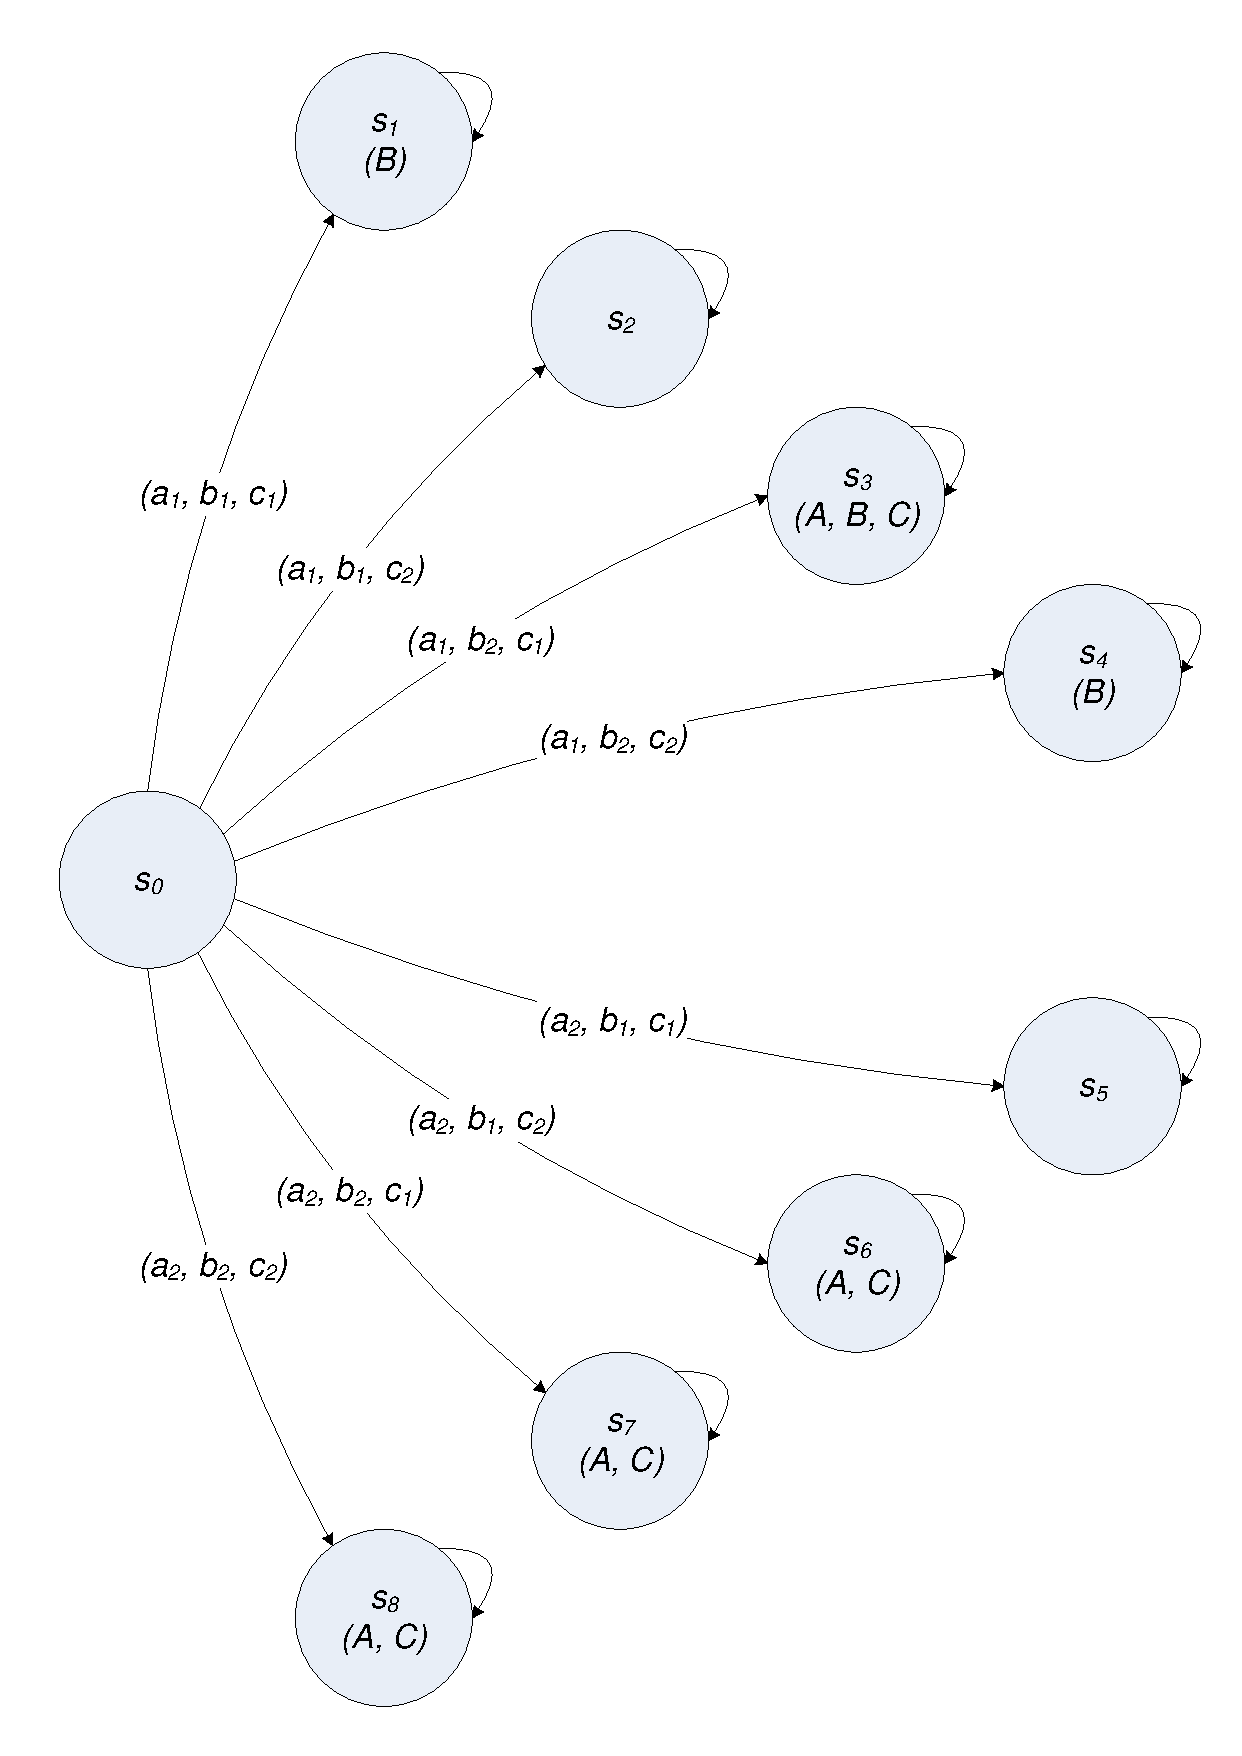
\includegraphics[scale=0.6]{ConcurrentGamepdf.pdf}
	\caption{A 3-player concurrent reachability game.}
	\label{fig:concurrentgame}
\end{figure}

\begin{remark}
Note that every \textit{k-resilient} Nash equilibrium is also a \textit{j-resilient} Nash equilibrium for every $j \leq k$.
\end{remark}

\begin{example}
Figure \ref{fig:matchingpennies} shows a two-player concurrent reachability game. There are three states in the game (labelled $s_{0}$ to $s_{2}$). The two players are $A_{1}$ and $A_{2}$. The actions allowed to both the players in state $s_{0}$ are $a$ and $b$. Edges are labelled with moves of players. A transition is applied when one of its labelled move is played. Edges (transitions) starting in states $s_{1}$ and $s_{2}$ are self loops and are not labelled with any move. The transitions that are not labelled with any move can be applied for every possible tuple of actions (move) of players. Some states are also labelled with names of players in brackets. If a player's name appears in brackets within a state label, it means that the reachability set of that player contains that state. Observe that $\Omega(A_{1}) = \lbrace s_{1} \rbrace$ and $\Omega(A_{2}) = \lbrace s_{2} \rbrace$.

From state $s_{0}$, if both the players choose the same action, the game goes to state $s_{1}$. If they choose different actions, the game goes to state $s_{2}$. Observe that this game does not exhibit any pure strategy Nash equilibrium (There does not exist a \textit{k-resilient} Nash equilibrium for any value of $k$).
\end{example}

\begin{figure}[H]
	\centering
	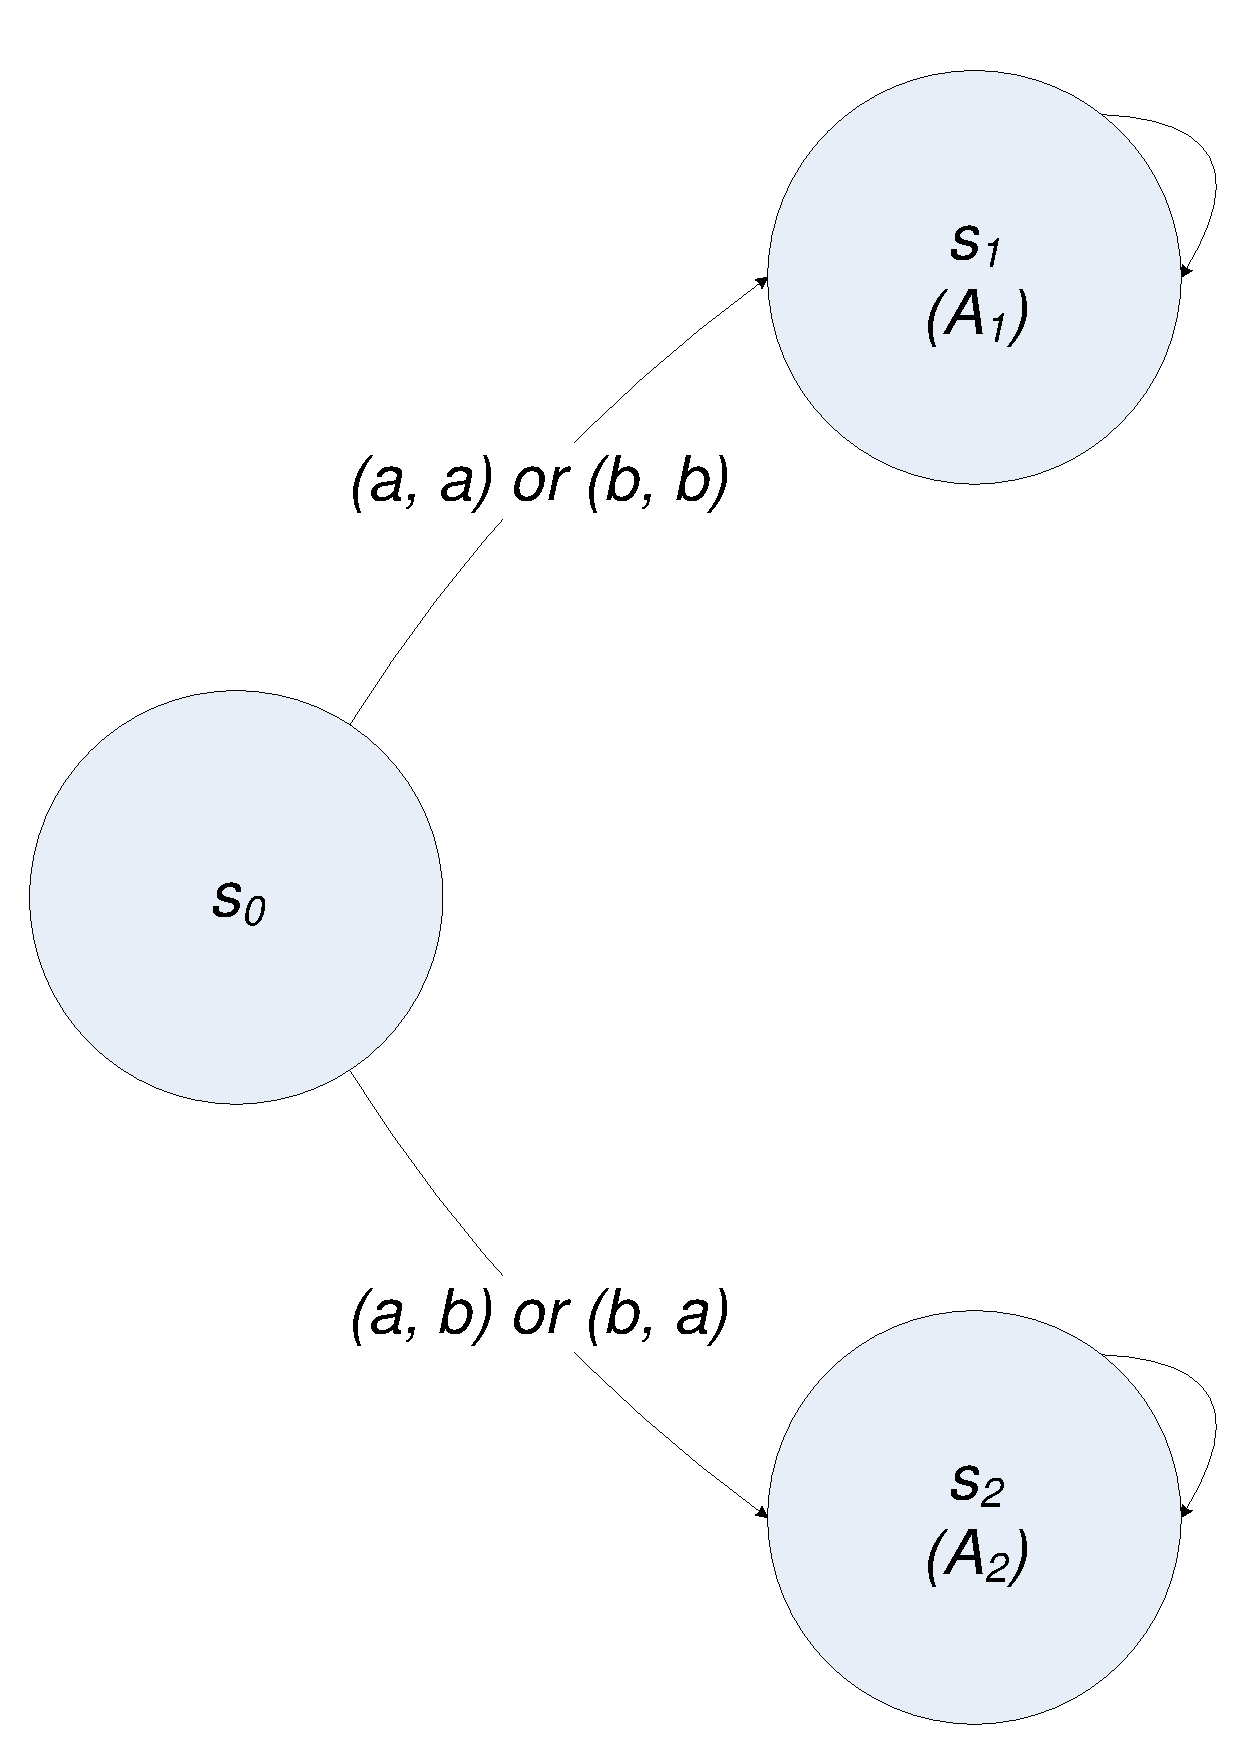
\includegraphics[scale=0.25]{MatchingPenniespdf.pdf}
	\caption{A 2-player concurrent reachability game.}
	\label{fig:matchingpennies}
\end{figure}

\begin{remark}
A \textit{k-resilient} Nash equilibrium may not necessarily exist in general.
\end{remark}

\section{Characterizing \textit{K-Resilient} Nash Equilibria}

In this section, we define the notion of \textit{k-suspect coalitions} and \textit{k-repellor sets} in non-deterministic multi-player concurrent reachability games. We then prove some properties associated with \textit{k-suspect coalitions} and \textit{k-repellor sets} that characterize \textit{k-resilient} Nash equilibria in these games. These properties are then used to develop the algorithm to check the existence of \textit{k-resilient} Nash equilibrium in finite non-deterministic multi-player concurrent reachability games. The properties that we prove also contain all the necessary information to compute a \textit{k-resilient} Nash equilibrium if it exists.

We now extend the definition of \textit{suspect players} given in \cite{BBM-concur10,BBM-report,BBMU-fsttcs11,Romain-phd} to \textit{k-suspect coalitions}.

\begin{definition}
In a game $G$, for some $k \leq \vert Agt \vert$, the set of \textit{k-suspect coalitions} for an edge $e = (s, s')$, given a move $m_{Agt}$ (denoted as $k-Susp_{G}(e, m_{Agt})$) is defined as the set:
\begin{align*}
k-Susp_{G}(e, m_{Agt}) &= \lbrace P \in 2^{Agt}_{k} \; \vert \; \forall B \in P. \; \exists m'_{B} \in Mov(s, B) \\
&\qquad s.t. \; e \in Tab(s, m_{Agt}[P \rightarrow m'_{P}])\\
&\qquad \text{where} \; m'_{P} = (m'_{B})_{B\in P} \; \text{is an action tuple for} \; P \rbrace
\end{align*}
\end{definition}

Intuitively, in a game $G$, a coalition $P$ of size at most $k$ is a \textit{k-suspect coalition} for an edge $e$, given a move $m_{Agt}$ (i.e., $P \in k-Susp_{G}(e, m_{Agt})$), whenever players of $P$ can deviate from their corresponding actions in $m_{Agt}$ (while other actions in $m_{Agt}$ are unchanged) and can take edge $e$ (i.e., players of $P$ can deviate from their corresponding actions in $m_{Agt}$ in such a way that edge $e$ is one of the possible transitions).

\begin{remark}
For an edge $e = (s, s')$, given a move $m_{Agt}$, if $e \in Tab(s, m_{Agt})$ then $k-Susp_{G}(e, m_{Agt}) = 2^{Agt}_{k}$.
\end{remark}

\begin{definition}
In a game $G$, for some $k \leq \vert Agt \vert$, the set of \textit{k-suspect coalitions} for a finite path $\pi = (s_{i})_{i \leq \vert \pi \vert}$, given a strategy profile $\sigma_{Agt}$ (denoted as $k-Susp_{G}(\pi, \sigma_{Agt})$) is defined as the set:
\begin{align*}
k-Susp_{G}(\pi, \sigma_{Agt}) = \bigcap \limits_{i<\vert \pi \vert} k-Susp_{G}((s_{i}, s_{i+1}), (\sigma_{A}(\pi_{\leq i}))_{A\in Agt})
\end{align*}
\end{definition}

\begin{lemma}
\label{lemma1}
In a game $G$, for some $k \leq \vert Agt \vert$, given $\sigma_{Agt} \in Strat^{Agt}_{G}$, $\pi \in Hist_{G}$ and a coalition $P$ of size at most $k$ ($P \in 2^{Agt}_{k}$), the following three propositions are equivalent:

(a) $P \in k-Susp_{G}(\pi, \sigma_{Agt})$

(b) $\exists \sigma'_{P} \in Strat^{P}_{G}. \; \pi \in Out_{G}^{f}(\sigma_{Agt}[P \rightarrow \sigma'_{P}])$

(c) $\pi \in Out_{G}^{f}((\sigma_{A})_{A\in Agt\setminus P})$
\end{lemma}

\begin{proof}
Propositions \textit{(b)} and \textit{(c)} are trivially equivalent. We prove here, the equivalence of propositions \textit{(a)} and \textit{(b)} which proves the lemma.

\textit{(a)} $\Rightarrow$ \textit{(b)}:

Let $\pi = (s_{i})_{i\leq \vert \pi \vert}$ and $P \in k-Susp_{G}(\pi, \sigma_{Agt})$. By definition of $k-Susp_{G}(\pi, \sigma_{Agt})$, for every $i < \vert \pi \vert$, $P \in k-Susp_{G}((s_{i}, s_{i+1}), (\sigma_{A}(\pi_{\leq i}))_{A\in Agt})$. For every $i < \vert \pi \vert$, let $(\sigma_{A}(\pi_{\leq i}))_{A\in Agt}$ denote the move $m_{Agt^{i}}$ ($m_{Agt^{i}} = (m_{A^{i}})_{A\in Agt}$). Now for every $i < \vert \pi \vert$, it holds that:
\begin{align*}
&\forall B \in P. \; \exists m'_{B^{i}} \in Mov(s_{i}, B) \; s.t. \; (s_{i}, s_{i+1}) \in Tab(s_{i}, m_{Agt^{i}}[P \rightarrow m'_{P^{i}}])\\
&\text{where} \; m'_{P^{i}} = (m'_{B^{i}})_{B\in P}
\end{align*}

We now define a strategy $\sigma'_{P}$ for the coalition $P$ as follows. For every $i < \vert \pi \vert$ and for every $B \in P$, let $\sigma'_{B}(\pi_{\leq i}) = m'_{B^{i}}$ and let $\sigma'_{P} = (\sigma'_{B})_{B\in P}$. For this $\sigma'_{P}$, we have:
\begin{align*}
\pi \in Out_{G}^{f}(\sigma_{Agt}[P \rightarrow \sigma'_{P}])
\end{align*}

\textit{(b)} $\Rightarrow$ \textit{(a)}:

Let $\pi = (s_{i})_{i\leq \vert \pi \vert}$ and let $\sigma'_{P} = (\sigma'_{B})_{B \in P}$. For every $i < \vert \pi \vert$, let $m_{Agt^{i}} = (\sigma_{A}(\pi_{\leq i}))_{A\in Agt}$ and let $m'_{P^{i}} = (\sigma'_{B}(\pi_{\leq i}))_{B\in P}$.

From \textit{(b)}, We have $\pi \in Out_{G}^{f}(\sigma_{Agt}[P \rightarrow \sigma'_{P}])$. Thus for every $i < \vert \pi \vert$, we have:
\begin{align*}
&\qquad & &(s_{i}, s_{i+1}) \in Tab(s_{i}, m_{Agt^{i}}[P \rightarrow m'_{P^{i}}])\\
&\Rightarrow & &P \in k-Susp_{G}((s_{i}, s_{i+1}), m_{Agt^{i}})\\
&\Rightarrow & &P \in k-Susp_{G}((s_{i}, s_{i+1}), (\sigma_{A}(\pi_{\leq i}))_{A\in Agt})
\end{align*}

As this is true for every $i < \vert \pi \vert$, we have:
\begin{align*}
&\qquad & &P \in \bigcap \limits_{i<\vert \pi \vert} k-Susp_{G}((s_{i}, s_{i+1}), (\sigma_{A}(\pi_{\leq i}))_{A\in Agt})\\
&\Rightarrow & &P \in k-Susp_{G}(\pi, \sigma_{Agt})
\end{align*}
\end{proof}

Intuitively, Lemma \ref{lemma1} states that in a game $G$, a coalition $P$ of size at most $k$ is a \textit{k-suspect coalition} for a path $\pi$, given a strategy profile $\sigma_{Agt}$ (i.e., $P \in k-Susp_{G}(\pi, \sigma_{Agt})$), whenever the coalition $P$ has a strategy to enforce the path $\pi$ under the strategies $(\sigma_{A})_{A\in Agt\setminus P}$ of the players not in $P$ (i.e., players of $P$ can deviate from their corresponding strategies in $\sigma_{Agt}$ in such a way that path $\pi$ is one of the possible outcomes).

\begin{remark}
For a finite path $\pi$, given a strategy profile $\sigma_{Agt}$, if $\pi \in Out_{G}^{f}(\sigma_{Agt})$ then $k-Susp_{G}(\pi, \sigma_{Agt}) = 2^{Agt}_{k}$.
\end{remark}

In a game $G$, for some $k \leq \vert Agt \vert$, consider the set of ordered pairs $(P, X)$ where $P \subseteq Agt$ is a coalition and $X \subseteq 2^{Agt}_{k}$ ($X$ is a subset of the set of all subsets of $Agt$ of size at most $k$). Let us define a partial ordering on the set of ordered pairs $(P, X)$ as follows:
\[(P', X') \leq (P, X) \; \textit{iff} \; P' \subseteq P \; \textit{and} \; X' \subseteq X\]

The relation `$\leq$' is trivially reflexive, transitive and anti-symmetric.

We now extend the definition of \textit{repellor sets} given in \cite{BBM-concur10,BBM-report,BBMU-fsttcs11} to \textit{k-repellor sets}.

\begin{definition}
\label{k-rep}
In a game $G$, for some $k \leq \vert Agt \vert$, given $P \subseteq Agt$ and $X \subseteq 2^{Agt}_{k}$, the \textit{k-repellor set} of the ordered pair $(P, X)$ (denoted as $k-Rep_{G}(P, X)$) is defined inductively as follows: as the base case, we let $k-Rep_{G}(\emptyset, X) = States$ for every $X \subseteq 2^{Agt}_{k}$. Then assuming that $k-Rep_{G}(P', X')$ has been defined for every $(P', X') \lneq (P, X)$, we let $k-Rep_{G}(P, X)$ be the largest set satisfying the following two conditions:

(a) $\forall B \in P. \; k-Rep_{G}(P, X) \cap \Omega(B) = \emptyset$

(b) $\forall s \in k-Rep_{G}(P, X). \; \exists m_{Agt} \in Act^{Agt}. \; \forall s' \in States. \; s' \in k-Rep_{G}(P', X')$

where $X' = k-Susp_{G}((s, s'), m_{Agt}) \cap X$ and $P' = P \bigcap \left( \bigcup \limits_{W \in X'}W \right)$
\end{definition}

Intuitively, in a game $G$, for some $k \leq \vert Agt \vert$, given $P \subseteq Agt$ and $X \subseteq 2^{Agt}_{k}$, $k-Rep_{G}(P, X)$ is the set of states from where players can cooperate to stay in $k-Rep_{G}(P, X)$, thus never satisfying the objectives of players in $P$, such that if any coalition $Q \in X$ deviates from its strategy and breaks the cooperation, it won't help fulfilling the objectives of players in $P \cap Q$ (i.e, if a coalition $Q \in X$ deviates and breaks the cooperation, the players of $Q$ which are also in $P$ can't be benefited). Intuitively, in $k-Rep_{G}(P, X)$, $P$ is the set of players whose objectives must not be fulfilled by deviations from coalitions in $X$.

\begin{lemma}
\label{lemma2}
In a game $G$, for some $k \leq \vert Agt \vert$, given $P, Q \subseteq Agt$ and $X, Y \subseteq 2^{Agt}_{k}$. If $Q \subseteq P$ and $Y \subseteq X$, then $k-Rep_{G}(P, X) \subseteq k-Rep_{G}(Q, Y)$.
\end{lemma}

\begin{proof}
We prove this lemma by induction on the ordered pair $(P, X)$.

Base case: $k-Rep_{G}(\emptyset, \emptyset) = States$. Hence, base case is trivial.

Inductive step: For some $(P, X)$, assume that the result holds for every $(P', X') \leq (P, X)$. We now need to prove that the result also holds for $(P, X)$.

Now consider $Q \subseteq P$, and $Y \subseteq X$ and consider the set $k-Rep_{G}(P, X)$. We prove that $k-Rep_{G}(P, X) \subseteq k-Rep_{G}(Q, Y)$ by showing that every state $s \in k-Rep_{G}(P, X)$ satisfies both the conditions (a) and (b) of Definition \ref{k-rep} to be in $k-Rep_{G}(Q, Y)$.

(a) Every $B \in Q$ is also in $P$. Therefore, we have:
\[\forall s \in k-Rep_{G}(P, X). \; \forall B \in Q. \; s \notin \Omega(B)\]

(b) For every $s \in k-Rep_{G}(P, X)$, there exists a move $m_{Agt}$, such that every state $s' \in States$ satisfies:

\[s' \in k-Rep_{G}(P', X')\]

where $X' = k-Susp_{G}((s, s'), m_{Agt}) \cap X$ and $P' = P \bigcap \left( \bigcup \limits_{W \in X'}W \right)$.

Here, $X' \subseteq X$ and $P' \subseteq P$. Therefore we have $(P', X') \leq (P, X)$. So, we can apply induction hypothesis on $(P', X')$.

Let $X'' = k-Susp_{G}((s, s'), m_{Agt}) \cap Y$ and let $P'' = Q \bigcap \left( \bigcup \limits_{W \in X''}W \right)$.

Clearly $X'' \subseteq X'$ and $P'' \subseteq P'$. Applying induction hypothesis on $(P', X')$, we get:
\begin{align*}
&\qquad & k-Rep_{G}(P', X') &\subseteq k-Rep_{G}(P'', X'')\\
&\Rightarrow & s' &\in k-Rep_{G}(P'', X'')
\end{align*}

where $X'' = k-Susp_{G}((s, s'), m_{Agt}) \cap Y$ and $P'' = Q \bigcap \left( \bigcup \limits_{W \in X''}W \right)$.

We have shown that every state $s \in k-Rep_{G}(P, X)$ satisfies both the conditions (a) and (b) of Definition \ref{k-rep} to be in $k-Rep_{G}(Q, Y)$. Therefore $k-Rep_{G}(P, X) \subseteq k-Rep_{G}(Q, Y)$ 
\end{proof}

We now extend the definition of \textit{secure moves} given in \cite{BBM-concur10,BBM-report} to \textit{k-secure moves}.

\begin{definition}
\label{k-securemove}
In a game $G$, for some $k \leq \vert Agt \vert$, given $P \subseteq Agt$, $X \subseteq 2^{Agt}_{k}$ and a state $s$, the set of \textit{k-secure moves} for the tuple $(s, P, X)$ (denoted as $k-Secure_{G}(s, P, X)$) is defined as:

$k-Secure_{G}(s, P, X) = \bigg\lbrace m_{Agt} \in Act^{Agt} \; \bigg\vert \; \forall s' \in States. \; s' \in k-Rep_{G}(P', X')$

where $X' = k-Susp_{G}((s, s'), m_{Agt}) \cap X$ and $P' = P \bigcap \left( \bigcup \limits_{W \in X'}W \right)\bigg\rbrace$
\end{definition}

Intuitively, $k-Secure_{G}(s, P, X)$ is the set of moves available from state $s \in k-Rep_{G}(P, X)$ for staying in $k-Rep_{G}(P, X)$ (hence the word \textit{k-secure}).

\textit{\textbf{A special case:}} In a game $G$, for some $k \leq \vert Agt \vert$, given $P \subseteq Agt$, $X \subseteq 2^{Agt}_{k}$ and a state $s$. If $P \bigcap \left( \bigcup \limits_{W \in X}W \right) \neq P$ (i.e., there is at least one player in $P$ which is not a member of any coalition in $X$), then playing a \textit{k-secure move} from $k-Rep_{G}(P, X)$ may take us outside $k-Rep_{G}(P, X)$. This may happen as follows: if a \textit{k-secure move} $m_{Agt} \in k-Secure_{G}(s, P, X)$ is played and a transition $(s, s')$ is applied as a result, then according to condition (b) of Definition \ref{k-rep}:
\begin{align*}
&\qquad & s' &\in k-Rep_{G}(P', X')\\
&\text{where} & X' &= k-Susp_{G}((s, s'), m_{Agt}) \cap X\\
&\Rightarrow & X' &= 2^{Agt}_{k} \cap X\\
&\Rightarrow & X' &= X\\
&\text{and} & P' &= P \bigcap \left( \bigcup \limits_{W \in X'}W \right)\\
&\Rightarrow & P' &= P \bigcap \left( \bigcup \limits_{W \in X}W \right)\\
&\Rightarrow & P' &\neq P \; (\text{as} \; P' \subsetneq P)
\end{align*}

Therefore, $s' \in k-Rep_{G}(P', X)$ but $s'$ is not necessarily in $k-Rep_{G}(P, X)$. From Lemma \ref{lemma2}, we have $k-Rep_{G}(P, X) \subseteq k-Rep_{G}(P', X)$. Therefore, $s'$ may or may not belong to $k-Rep_{G}(P, X)$. Thus, taking a \textit{k-secure move} from $k-Rep_{G}(P, X)$ in such cases does not necessarily mean staying in $k-Rep_{G}(P, X)$. Although, this seems to violate our intuitive meaning of \textit{k-secure moves}, this is not something undesirable. Its just a special case. This happens because there is at least one player $B \in P$ which is not a member of any coalition in $X$. Therefore if $s \in k-Rep_{G}(P, X)$, then $s \notin \Omega(B)$. But after a \textit{k-secure move} $m_{Agt}$ is played resulting in the transition $(s, s')$, $B$ may then be allowed to fulfil its objective ($s'$ may belong to $\Omega(B)$) according to the definition (as $B$ is not a member of any coalition in $X$).

This special case does not affect our results because, in this thesis, we will only be considering the cases where $P \bigcap \left( \bigcup \limits_{W \in X}W \right) = P$ (i.e., every player in $P$ is a member of at least one coalition in $X$). In such cases taking a \textit{k-secure move} from $k-Rep_{G}(P, X)$ results in staying in $k-Rep_{G}(P, X)$ as expected according to the intuitive meaning of \textit{k-secure moves}.

\begin{definition}
\label{k-spx}
In a game $G$, for some $k \leq \vert Agt \vert$, given $P \subseteq Agt$ and $X \subseteq 2^{Agt}_{k}$, we define the transition system $k-S_{G}(P, X) = (States, Edg')$ as follows: $(s, s') \in Edg'$ iff there exists some move $m_{Agt} \in k-Secure_{G}(s, P, X)$ such that $(s, s') \in Tab(s, m_{Agt})$. Note in particular that every $s \in k-Rep_{G}(P, X)$ has an outgoing transition in $k-S_{G}(P, X)$.
\end{definition}

\begin{lemma}
\label{lemma3}
In a game $G$, for some $k \leq \vert Agt \vert$, given $s \in States$, $P \subseteq Agt$ and $X \subseteq 2^{Agt}_{k}$ such that $P \bigcap \left( \bigcup \limits_{W \in X}W \right) = P$. Then $s \in k-Rep_{G}(P, X)$ if and only if there exists an infinite path $\pi$ in $k-S_{G}(P, X)$ starting from $s$.
\end{lemma}

\begin{proof}
($\Rightarrow$) We construct $\pi = (s_{i})_{i\geq 0}$ inductively starting with $s_{0} = s$. Then assuming that $s_{i} \in k-Rep_{G}(P, X)$ for some $i$, we can define $s_{i+1}$ to be such that $(s_{i}, s_{i+1})$ corresponds to a \textit{k-secure move} $m_{Agt} \in k-Secure_{G}(s_{i}, P, X)$. Then we have:
\begin{align*}
&\qquad & s_{i+1} &\in k-Rep_{G}(P', X')\\
&\text{where} & X' &= k-Susp_{G}((s_{i}, s_{i+1}), m_{Agt}) \cap X\\
&\Rightarrow & X' &= 2^{Agt}_{k} \cap X\\
&\Rightarrow & X' &= X\\
&\text{and} & P' &= P \bigcap \left( \bigcup \limits_{W \in X'}W \right)\\
&\Rightarrow & P' &= P \bigcap \left( \bigcup \limits_{W \in X}W \right)\\
&\Rightarrow & P' &= P
\end{align*}

Therefore $s_{i+1} \in k-Rep_{G}(P, X)$. This holds for every $i \geq 0$. Hence $\pi$ is an infinite path in $k-S_{G}(P, X)$.

($\Leftarrow$) Writing $\pi = (s_{i})_{i\geq 0}$, by construction of transition system $k-S_{G}(P, X)$, we have $(s_{0}, s_{1}) \in Tab(s_{0}, m_{Agt})$ for some $m_{Agt} \in k-Secure_{G}(s_{0}, P, X)$. Therefore $s_{0} \in k-Rep_{G}(P, X)$ which means $s \in k-Rep_{G}(P, X)$.
\end{proof}

We now recall the following lemma from \cite{BBM-report}. The proof of the following lemma is same as in \cite{BBM-report}.

\begin{lemma}
\label{lemma4}
In a game $G$, let $P \subseteq Agt$ be a coalition and let $\sigma_{P} \in Strat^{P}_{G}$ be a strategy for coalition $P$ ($\sigma_{P} = (\sigma_{A})_{A \in P}$). Let $s \in States$ and $\pi \in Out^{f}_{G}(s, \sigma_{P})$ ending in some state $s'$. For any history $\tau$ starting in $s'$, define $\sigma_{A}^{-\pi}(\tau) = \sigma_{A}(\pi \cdot \tau)$. Then
\[\pi \cdot Out_{G}(s', (\sigma_{A}^{-\pi})_{A\in P}) \subseteq Out_{G}(s, \sigma_{P})\]
\end{lemma}

\begin{proof}
Let $\pi' \in \pi \cdot Out_{G}(s', (\sigma_{A}^{-\pi})_{A\in P})$. Let us write $\pi = (s_{i})_{i\leq \vert \pi \vert}$ and $\pi' = (s'_{i})_{i\leq \vert \pi' \vert}$.

If $i < \vert \pi \vert$, then $(s'_{i}, s'_{i+1}) = (s_{i}, s_{i+1})$, so that $(s'_{i}, s'_{i+1}) \in Tab(s'_{i}, m_{Agt^{i}})$ for some move $m_{Agt^{i}} = (m_{A^{i}})_{A \in Agt}$ such that $m_{A^{i}} = \sigma_{A}(\pi_{\leq i})$ for every $A \in P$.

Otherwise, if $i \geq \vert \pi \vert$, let $\rho$ be the path such that $\pi \cdot \rho = \pi'_{\leq i}$. Then $(s'_{i}, s'_{i+1}) \in Tab(s'_{i}, m'_{Agt^{i}})$ for some move $m'_{Agt^{i}} = (m'_{A^{i}})_{A\in Agt}$ such that $m'_{A^{i}} = \sigma_{A}^{-\pi}(\rho)$ for every $A \in P$. Therefore $m'_{A^{i}} = \sigma_{A}(\pi \cdot \rho) = \sigma_{A}(\pi'_{\leq i})$ for every $A \in P$.

Hence $\pi' \in Out_{G}(s, (\sigma_{A})_{A\in P})$. Hence $\pi \cdot Out_{G}(s', (\sigma_{A}^{-\pi})_{A\in P}) \subseteq Out_{G}(s, \sigma_{P})$.
\end{proof}

\begin{lemma}
\label{lemma5}
In a game $G$, for some $k \leq \vert Agt \vert$, given $s \in States$, $P \subseteq Agt$ and $X \subseteq 2^{Agt}_{k}$ such that $P \bigcap \left( \bigcup \limits_{W \in X}W \right) = P$. Let $\pi \in Play_{G}(s)$ be an infinite play with initial state $s$. Then $\pi$ is a path in $k-S_{G}(P, X)$ if and only if there exists $\sigma_{Agt} \in Strat^{Agt}_{G}$ such that $\pi \in Out_{G}(s, \sigma_{Agt})$ and for every $Q \in X$ and every $\sigma'_{Q} \in Strat^{Q}_{G}$, it holds that:

$\forall \pi' \in Out_{G}(s, \sigma_{Agt}[Q \rightarrow \sigma'_{Q}]). \; \pi'$ does not visit $\Omega(B)$ for every $B \in P \cap Q$.
\end{lemma}

\begin{proof}
($\Rightarrow$) Assume that $\pi = (s_{i})_{i\geq 0}$ is an infinite play in $k-S_{G}(P, X)$. Let us define the following partial functions:

(i) $c: States \times 2^{Agt} \times 2^{2^{Agt}_{k}} \rightarrow Act^{Agt}$: for every tuple $(s, R, Y)$ such that $s \in k-Rep_{G}(R, Y)$, we let $c(s, R, Y) = m_{Agt}$ for some move $m_{Agt} \in k-Secure_{G}(s, R, Y)$.

(ii) $d: \mathbb{N} \rightarrow Act^{Agt}$: for every $i \in \mathbb{N}$, we let $d(i) = m_{Agt^{i}}$ for some move $m_{Agt^{i}} \in k-Secure_{G}(s_{i}, P, X)$ such that $(s_{i}, s_{i+1}) \in Tab(s_{i}, m_{Agt^{i}})$. This is well defined because $\pi$ is a play in $k-S_{G}(P, X)$.

The strategy profile $\sigma_{Agt}$ is defined as follows:

On prefixes of $\pi$, we let $\sigma_{A}(\pi_{\leq i}) = (d(i))(A)$ for every $i \in \mathbb{N}$, where $(d(i))(A)$ represents the action corresponding to the player $A$ in the move $d(i)$.

For any $\pi' = (s'_{i})_{i\leq \vert \pi' \vert}$ that is not a prefix of $\pi$, we let $\sigma_{A}(\pi') = (c(s'_{\vert \pi' \vert}, P', X'))(A)$ where $X' = k-Susp_{G}(\pi', \sigma_{Agt}) \cap X$, $P' = P \bigcap \left( \bigcup \limits_{W \in X'}W \right)$ and $(c(s'_{\vert \pi' \vert}, P', X'))(A)$ represents the action corresponding to the player $A$ in the move $c(s'_{\vert \pi' \vert}, P', X')$.

By construction, we have $\pi \in Out_{G}(s, \sigma_{Agt})$. Let $Q$ be a coalition in $X$ ($Q \in X$) and let $\sigma'_{Q}$ be a strategy for the coalition $Q$ ($\sigma'_{Q} \in Strat^{Q}_{G}$) such that $\sigma'_{Q} = (\sigma'_{B})_{B\in Q}$. Let $\pi' \in Out_{G}(s, \sigma_{Agt}[Q \rightarrow \sigma'_{Q}])$. Assuming $\pi' = (s'_{i})_{i\geq 0}$, we show by induction on $i$ that:
\[s'_{i} \in k-Rep_{G}(P \cap Q, \lbrace Q \rbrace) \; \text{for every} \; i \in \mathbb{N}\]

Base case: When $i = 0$, $s'_{0} = s$. We know that $\pi$ is a play in $k-S_{G}(P, X)$ starting from $s$. Therefore, from Lemma \ref{lemma3}, we get that $s \in k-Rep_{G}(P, X)$ which implies $s'_{0} \in k-Rep_{G}(P, X)$. As $P \cap Q \subseteq P$ and $\lbrace Q \rbrace \subseteq X$, from Lemma \ref{lemma2} we get $s'_{0} \in k-Rep_{G}(P \cap Q, \lbrace Q \rbrace)$. Hence base case is true.

Inductive step: Assume that for some $i \geq 0$, $s'_{i} \in k-Rep_{G}(P \cap Q, \lbrace Q \rbrace)$. Let $(\sigma_{A}(\pi'_{\leq i}))_{A\in Agt} = m_{Agt^{i}}$. Let $(\sigma'_{B}(\pi'_{\leq i}))_{B\in Q} = m'_{Q^{i}}$. By construction of $\pi'$, we have $(s'_{i}, s'_{i+1}) \in Tab(s'_{i}, m_{Agt^{i}}[Q \rightarrow m'_{Q^{i}}])$ which implies:
\begin{align*}
Q \in k-Susp_{G}((s'_{i}, s'_{i+1}), m_{Agt^{i}})
\end{align*}

If $\pi'_{\leq i}$ is not a prefix of $\pi$, then the strategy profile $\sigma_{Agt}$ is defined using $c$. Therefore, $(\sigma_{A}(\pi'_{\leq i}))_{A\in Agt} = m_{Agt^{i}} = c(s'_{i}, P', X')$ where $X' = k-Susp_{G}(\pi', \sigma_{Agt}) \cap X$ and $P' = P \bigcap \left( \bigcup \limits_{W \in X'}W \right)$. By definition, $s'_{i} \in k-Rep_{G}(P', X')$ and $m_{Agt^{i}} \in k-Secure_{G}(s'_{i}, P', X')$. From condition (b) of Definition \ref{k-rep}, we get that:
\[s'_{i+1} \in k-Rep_{G}(P'', X'')\]

where $X'' = k-Susp_{G}((s'_{i}, s'_{i+1}), m_{Agt^{i}}) \cap X'$ and $P'' = P' \bigcap \left( \bigcup \limits_{W \in X''}W \right)$

By construction of $\pi'$, we know that $Q \in k-Susp_{G}(\pi', \sigma_{Agt})$. And by induction hypothesis, $s'_{i} \in k-Rep_{G}(P \cap Q, \lbrace Q \rbrace)$. Therefore $\lbrace Q \rbrace \subseteq X'$ and $P \cap Q \subseteq P'$. Now as $Q \in k-Susp_{G}((s'_{i}, s'_{i+1}), m_{Agt^{i}})$, we get that $\lbrace Q \rbrace \subseteq X''$ and $P \cap Q \subseteq P''$. Therefore from Lemma \ref{lemma2}, we conclude that $s'_{i+1} \in k-Rep_{G}(P \cap Q, \lbrace Q \rbrace)$.

Now if $\pi'_{\leq i}$ is a prefix of $\pi$, then the strategy profile $\sigma_{Agt}$ is defined using $d$. Therefore, $(\sigma_{A}(\pi'_{\leq i}))_{A\in Agt} = m_{Agt^{i}} = d(s'_{i}, P, X)$. By definition, $s'_{i} \in k-Rep_{G}(P, X)$ and $m_{Agt^{i}} \in k-Secure_{G}(s'_{i}, P, X)$. From condition (b) of Definition \ref{k-rep}, we get that:
\[s'_{i+1} \in k-Rep_{G}(P'', X'')\]

where $X'' = k-Susp_{G}((s'_{i}, s'_{i+1}), m_{Agt^{i}}) \cap X$ and $P'' = P \bigcap \left( \bigcup \limits_{W \in X''}W \right)$.

Now as $Q \in k-Susp_{G}((s'_{i}, s'_{i+1}), m_{Agt^{i}})$, we get that $\lbrace Q \rbrace \subseteq X''$ and $P \cap Q \subseteq P''$. Therefore from Lemma \ref{lemma2}, we conclude that $s'_{i+1} \in k-Rep_{G}(P \cap Q, \lbrace Q \rbrace)$.

This proves the inductive step. Hence $\pi'$ does not visit $\Omega(B)$ for every $B \in P \cap Q$.

($\Leftarrow$) Let $\sigma_{Agt}$ be a strategy profile such that $\pi \in Out_{G}(s, \sigma_{Agt})$ and for every $Q \in X$ and every $\sigma'_{Q} \in Strat^{Q}_{G}$, it holds that:

$\forall \pi' \in Out_{G}(s, \sigma_{Agt}[Q \rightarrow \sigma'_{Q}]). \; \pi'$ does not visit $\Omega(B)$ for every $B \in P \cap Q$.

The proof for the implication is by induction on the ordered pair $(P, X)$.

Base case: If $P = \emptyset$, then by Definition \ref{k-rep}, $k-Rep_{G}(\emptyset, X) = States$ for every $X \subseteq 2^{Agt}_{k}$. Hence the result holds for the base case.

Inductive step: Let us assume that the implication is true for every $(P', X') \lneq (P, X)$ which satisfy the condition $P' \bigcap \left( \bigcup \limits_{W \in X'}W \right) = P'$.

We define the set:

$S = \lbrace s' \in States \; \vert \; \exists \rho \in Hist_{G}(s) \; \text{with} \; last(\rho) = s' \; \text{and} \; X \subseteq k-Susp_{G}(\rho, \sigma_{Agt}) \rbrace$

Let $s' \in S$ and $\rho \in Hist_{G}(s)$ be a history starting in $s$ such that $last(\rho) = s'$ and $X \subseteq k-Susp_{G}(\rho, \sigma_{Agt})$. According to Lemma \ref{lemma1}, any coalition $Q \in X$ has a strategy $\sigma'_{Q} \in Strat^{Q}_{G}$ such that $\rho \in Out^{f}_{G}(s, \sigma_{Agt}[Q \rightarrow \sigma'_{Q}])$. As a consequence $\rho$ does not visit $\Omega(B)$ for every $B \in P \cap Q$, which means $s \notin \Omega(B)$ and $s' \notin \Omega(B)$ for every $B \in P \cap Q$. This shows that for every $Q \in X$, it holds: $S \cap \Omega(B) = \emptyset$ for every $B \in P \cap Q$.

Let $m_{Agt} = (\sigma_{A}(\rho))_{A\in Agt}$ and $s'' \in States$. Then:

If $X \subseteq k-Susp_{G}((s', s''), m_{Agt})$, then $s'' \in S$.

Otherwise $X \cap k-Susp_{G}((s', s''), m_{Agt}) \subsetneq X$. We write $X'$ for this set and we let $P' = P \bigcap \left( \bigcup \limits_{W \in X'}W \right)$. So $(P', X') \lneq (P, X)$ and we can apply  induction hypothesis on $(P', X')$. Pick a coalition $Q \in X'$ and let $\rho' = \rho \cdot s''$. According to Lemma \ref{lemma4}:
\[\rho' \cdot Out_{G}(s'', (\sigma_{A}^{-\rho'})_{A\in Agt\setminus Q}) \subseteq Out_{G}(s, \sigma_{Agt\setminus Q})\]

But, according to the given condition, any path in $Out_{G}(s, \sigma_{Agt\setminus Q})$ does not visit $\Omega(B)$ for every $B \in P \cap Q$. As $P' \subseteq P$, $\rho' \cdot Out_{G}(s'', (\sigma_{A}^{-\rho'})_{A\in Agt\setminus Q})$ does not visit $\Omega(B)$ for every $B \in P' \cap Q$. Applying induction hypothesis on $(P', X')$ and using Lemma \ref{lemma3}, we get $s'' \in k-Rep_{G}(P', X')$.

This proves that $S \subseteq k-Rep_{G}(P, X)$ (as any state $s' \in S$ satisfies both the conditions of Definition \ref{k-rep} to stay in $k-Rep_{G}(P, X)$) and the move $(\sigma_{A}(\rho))_{A\in Agt}$ belongs to $k-Secure_{G}(last(\rho), P, X)$. Since $\pi$ is an outcome of $\sigma_{Agt}$, $\pi$ involves playing \textit{k-secure moves} to stay in $k-Rep_{G}(P, X)$. Hence $\pi$ is a play in $k-S_{G}(P, X)$.
\end{proof}

\begin{theorem}
\label{theorem6}
Let $G$ be a non-deterministic multi-player concurrent reachability game and let $s \in States$. There is a \textit{k-resilient} pseudo-Nash equilibrium in $G$ from $s$ with a payoff vector $v_{Agt} = (v_{A})_{A\in Agt}$ if and only if, letting $P = \lbrace A \in Agt \; \vert \; v_{A} = 0 \rbrace$, there is an infinite path $\pi$ in $k-S_{G}(P, 2^{Agt}_{k})$ which starts in $s$ and visits $\Omega(A)$ for every $A \notin P$. Furthermore, $\pi$ is the k-optimal play for this \textit{k-resilient} pseudo-Nash equilibrium.
\end{theorem}

\begin{proof}
($\Rightarrow$) Let $(\sigma_{Agt}, \pi)$ be a \textit{k-resilient} pseudo-Nash equilibrium from $s$ with payoff vector $v_{Agt} = (v_{A})_{A\in Agt}$. This means $\sigma_{Agt}$ is a strategy profile and $\pi \in Out_{G}(s, \sigma_{Agt})$.

Let $P = \lbrace A \in Agt \; \vert \; v_{A} = 0 \rbrace$. Therefore $\pi$ visits $\Omega(A)$ for every $A \notin P$. 

Also, as $(\sigma_{Agt}, \pi)$ is a \textit{k-resilient} pseudo-Nash equilibrium, for every $Q \in 2^{Agt}_{k}$ and every $\sigma'_{Q} \in Strat^{Q}_{G}$, it holds that:
\[\forall \pi' \in Out_{G}(s, \sigma_{Agt}[Q \rightarrow \sigma'_{Q}]). \; \forall B \in Q. \; v_{B}(\pi') \leq v_{B}(\pi)\]

But $v_{B}(\pi) = 0$ for every $B \in P$ which means $v_{B}(\pi) = 0$ for every $B \in P \cap Q$. This implies $v_{B}(\pi') = 0$ for every $B \in P \cap Q$ or the path $\pi'$ does not visit $\Omega(B)$ for every $B \in P \cap Q$.

Therefore, we have that, for every $Q \in 2^{Agt}_{k}$ and every $\sigma'_{Q} \in Start^{Q}_{G}$, it holds:

$\forall \pi' \in Out_{G}(s, \sigma_{Agt}[Q \rightarrow \sigma'_{Q}]). \; \pi'$ does not visit $\Omega(B)$ for every $B \in P \cap Q$.

By Lemma \ref{lemma5}, we get that $\pi$ must be a path in $k-S_{G}(P, 2^{Agt}_{k})$.

($\Leftarrow$) Let $\pi$ be an infinite path in $k-S_{G}(P, 2^{Agt}_{k})$ such that $\pi$ visits $\Omega(A)$ for every $A \notin P$. 

As $\pi$ is a play in $k-S_{G}(P, 2^{Agt}_{k})$, according to Lemma \ref{lemma5} there is a strategy profile $\sigma_{Agt} \in Strat^{Agt}_{G}$ such that, $\pi \in Out_{G}(s, \sigma_{Agt})$ and for every $Q \in 2^{Agt}_{k}$ and every $\sigma'_{Q} \in Strat^{Q}_{G}$, it holds:

$\forall \pi' \in Out_{G}(s, \sigma_{Agt}[Q \rightarrow \sigma'_{Q}]). \; \pi'$ does not visit $\Omega(B)$ for every $B \in P \cap Q$.

Therefore, we have that, for every $Q \in 2^{Agt}_{k}$ and every $\sigma'_{Q} \in Strat^{Q}_{G}$, it holds:
\[\forall \pi' \in Out_{G}(s, \sigma_{Agt}[Q \rightarrow \sigma'_{Q}]). \; \forall B \in Q. \; v_{B}(\pi') \leq v_{B}(\pi)\]

Hence $(\sigma_{Agt}, \pi)$ is a \textit{k-resilient} pseudo-Nash equilibrium.
\end{proof}

Theorem \ref{theorem6} gives a necessary and sufficient condition for existence of a \textit{k-resilient} pseudo-Nash equilibrium in a game $G$. In case a \textit{k-resilient} pseudo-Nash equilibrium exists, the \textit{k-repellor} sets and the corresponding transition systems contain all the necessary information to compute the equilibrium. The following theorem gives a generic method to compute a \textit{k-resilient} pseudo-Nash equilibrium if it exists.

\begin{theorem}
\label{theorem7}
In a game $G$, if $\pi$ is an infinite path in $k-S_{G}(P, 2^{Agt}_{k})$ from a state $s$ visiting $\Omega(A)$ for every $A \notin P$, then there is a \textit{k-resilient} pseudo-Nash equilibrium $(\sigma_{Agt}, \pi)$ where the strategy profile $\sigma_{Agt}$ consists in playing \textit{k-secure moves} in the transition system $k-S_{G}(P \cap P', 2^{Agt}_{k} \cap X')$ for some $P' \subseteq Agt$ and $X' \subseteq 2^{Agt}_{k}$ satisfying the condition $(P \cap P') \bigcap \left( \bigcup \limits_{W \in 2^{Agt}_{k} \cap X'}W \right) = (P \cap P')$.
\end{theorem}

\begin{proof}
For every $P \subseteq Agt$ and every $X \subseteq 2^{Agt}_{k}$ such that $P \bigcap \left( \bigcup \limits_{W \in X}W \right) = P$ and for every $s \in k-Rep_{G}(P, X)$, there is a \textit{k-secure move} $m_{Agt} \in k-Secure_{G}(s, P, X)$ such that every $(s, s') \in Tab(s, m_{Agt})$ is an edge of $k-S_{G}(P, X)$ (Lemma \ref{lemma3}). For every $P \subseteq Agt$ and every $X \subseteq 2^{Agt}_{k}$ such that $P \bigcap \left( \bigcup \limits_{W \in X}W \right) = P$, let us define memoryless strategies $\sigma_{Agt}^{P, X}$ which select such a \textit{k-secure move} to stay in $k-Rep_{G}(P, X)$. For every $s \in k-Rep_{G}(P, X)$, every $\pi \in Out_{G}(s, \sigma_{Agt}^{P, X})$ is a path in $k-S_{G}(P, X)$. The idea is that as soon as any coalition $Q \in X$ deviates, we compute the sets $X' = X \cap k-Susp_{G}((s, s'), \sigma_{Agt}^{P, X})$ and $P' = P \bigcap \left( \bigcup \limits_{W \in X'}W \right)$ and then we play strategies $\sigma_{Agt}^{P', X'}$ so that the players of the deviating coalition which are also in $P$ can't benefit.

Let $\pi = (s_{i})_{i\geq 0}$ be an infinite path in $k-S_{G}(P, 2^{Agt}_{k})$ that starts in state $s$ and visits $\Omega(A)$ for every $A \notin P$. The strategy profile $\sigma_{Agt}$ aims at playing $\pi$, and if any coalition $Q \in 2^{Agt}_{k}$ deviates, the strategies will be computed as mentioned earlier. Therefore, we define the strategy profile $\sigma_{Agt}$ as follows: 

For every history $\pi' = (s'_{i})_{i\leq m}$ in the game, we distinguish between several cases:
\begin{enumerate}
\item If $\pi'$ is a prefix of $\pi$ ($s'_{i} = s_{i}$ if $i \leq m$), then we define $(\sigma_{A}(\pi'))_{A\in Agt}$ as a \textit{k-secure move} with respect to $(P, 2^{Agt}_{k})$ such that $(s'_{m}, s_{m+1}) \in Tab(s'_{m}, (\sigma_{A}(\pi'))_{A\in Agt})$, so that the play continues in $\pi$.
\item If $\pi'$ is a path in $k-S_{G}(P, 2^{Agt}_{k})$ but not a prefix of $\pi$, then we define $(\sigma_{A}(\pi'))_{A\in Agt}$ as a \textit{k-secure move} with respect to $(P, 2^{Agt}_{k})$ from $last(\pi')$. This choice can be made memoryless and depends only on $last(\pi')$.
\item Otherwise decompose $\pi'$ as $\pi_{1} \cdot \pi_{2} \cdot \pi_{3} \cdots \pi_{l}$ such that there exist $P_{l} \subseteq P_{l-1} \cdots \subseteq P_{2} \subseteq P$ and $X_{l} \subseteq X_{l-1} \cdots \subseteq X_{2} \subseteq 2^{Agt}_{k}$ with:
\begin{enumerate}
\item $\pi_{1}$ is a path in $k-S_{G}(P, 2^{Agt}_{k})$.
\item If $1 < j \leq l$, then $\pi_{j}$ is a path in $k-S_{G}(P \cap P_{j}, 2^{Agt}_{k} \cap X_{j})$.
\item $X_{2} = k-Susp_{G}((last(\pi_{1}), first(\pi_{2})), (\sigma_{A}(\pi_{1}))_{A\in Agt})$

and

$P_{2} = P \bigcap \left( \bigcup \limits_{W \in X_{2}}W \right)$.
\item If $1 < j < l$, then 

$X_{j+1} = X_{j} \cap k-Susp_{G}((last(\pi_{j}), first(\pi_{j+1})), (\sigma_{A}^{P_{j}, X_{j}}(last(\pi_{j})))_{A\in Agt})$

and

$P_{j+1} = P_{j} \bigcap \left( \bigcup \limits_{W \in X_{j+1}}W \right)$.
\end{enumerate}
And we define $\sigma_{A}(\pi')$ as $\sigma_{A}^{P_{l}, X_{l}}(last(\pi'))$.
\end{enumerate}

We claim that $(\sigma_{Agt}, \pi)$ is a \textit{k-resilient} pseudo-Nash equilibrium. It is given that $\pi$ visits $\Omega(A)$ for every $A \notin P$. If $v_{Agt} = (v_{A})_{A\in Agt}$ is the payoff vector associated with $\pi$, then $v_{A}(\pi) = 1$ for every $A \notin P$ and $v_{A}(\pi) = 0$ for every $A \in P$. Now suppose a coalition $Q \in 2^{Agt}_{k}$ deviates and follows strategy $\sigma'_{Q}$. Then for every $\pi' \in Out_{G}(s, \sigma_{Agt}[Q \rightarrow \sigma'_{Q}])$, we can decompose $\pi'$ as $\pi_{1} \cdot \pi_{2} \cdot \pi_{3} \cdots \pi_{l}$ as described above. Also, as the coalition $Q$ deviated from its strategy resulting in the path $\pi'$, $Q \in k-Susp_{G}(\pi', \sigma_{Agt})$. Hence $Q \in X_{j}$ for every $1 \leq j \leq l$. This implies that for every $1 \leq j \leq l$, $\pi_{j}$ does not visit $\Omega(B)$ for every $B \in P_{j} \cap Q$. Therefore the path $\pi'$ does not visit $\Omega(B)$ for every $B \in P \cap Q$.

Therefore, we have that, for every $Q \in 2^{Agt}_{k}$ and every $\sigma'_{Q} \in Strat^{Q}_{G}$, it holds:
\[\forall \pi' \in Out_{G}(s, \sigma_{Agt}[Q \rightarrow \sigma'_{Q}]). \; \forall B \in Q. \; v_{B}(\pi') \leq v_{B}(\pi)\]

Hence $(\sigma_{Agt}, \pi)$ is a \textit{k-resilient} pseudo-Nash equilibrium.
\end{proof}

\section{Application to Finite Games}

In this section, we provide the algorithm to check the existence of \textit{k-resilient} Nash equilibrium in finite non-deterministic multi-player concurrent reachability games when only pure strategies are allowed.

A finite non-deterministic multi-player concurrent reachability game is a game in which the underlying transition system ($(States, Edg)$) is finite and the set of actions ($Act$) is also finite.

Given a finite game $G$, a state $s$ in $G$ and a positive integer $k \leq \vert Agt \vert$, we can apply Theorem \ref{theorem6} to develop an algorithm for checking existence of a \textit{k-resilient} pseudo-Nash equilibrium in the game $G$ from state $s$.

\begin{algorithm}
\caption{Existence of a \textit{k-resilient} pseudo-Nash equilibrium in a game.}
\label{algorithm1}
\begin{algorithmic}[1]
\renewcommand{\algorithmicrequire}{\textbf{Input:}}
\renewcommand{\algorithmicensure}{\textbf{Output:}}
\REQUIRE A finite non-deterministic multi-player concurrent reachability game $G$, a state $s$ in $G$ and a positive integer $k \leq \vert Agt \vert$.
\ENSURE A boolean value: \TRUE $\;$if there exists a \textit{k-resilient} pseudo-Nash equilibrium in $G$ from $s$; \FALSE $\;$otherwise.
\FOR{every possible payoff vector $v_{Agt} = (v_{A})_{A\in Agt}$}
\STATE $P \leftarrow \lbrace A \in Agt \; \vert \; v_{A} = 0 \rbrace$
\STATE Compute $k-Rep_{G}(P, 2^{Agt}_{k})$
\STATE Construct $k-S_{G}(P, 2^{Agt}_{k})$
\FOR{every play $\pi$ in $k-S_{G}(P, 2^{Agt}_{k})$ starting from $s$}
\IF{$\pi$ visits $\Omega(A)$ for every $A \notin P$}
\RETURN \TRUE
\ENDIF
\ENDFOR
\ENDFOR
\RETURN \FALSE
\end{algorithmic}
\end{algorithm}

The correctness of Algorithm \ref{algorithm1} follows from Theorem \ref{theorem6}.

\textit{\textbf{Time complexity analysis}}: In Algorithm \ref{algorithm1}, the loop of step 1 runs $2^{\vert Agt \vert}$ times (as the number of possible payoff vectors is $2^{\vert Agt \vert}$). In step 2, construction of the set $P$ involves checking $v_{A}$ for every $A \in Agt$. Hence step 2 takes O($\vert Agt \vert$) time. Step 3 and step 4 involve computation of $k-Rep_{G}(P, 2^{Agt}_{k})$ and construction of $k-S_{G}(P, 2^{Agt}_{k})$ respectively. This can be achieved by filling a table $R(s', Q, Y)$ for every $s' \in States$, every $Q \subseteq Agt$ and every $Y \subseteq 2^{Agt}_{k}$ such that $R(s', Q, Y) = 1$ if $s' \in k-Rep_{G}(Q, Y)$ and $R(s', Q, Y) = 0$ otherwise. This table can be filled inductively. As the base step, we let $R(s', \emptyset, Y) = 1$ for every $s' \in States$ and every $Y \subseteq 2^{Agt}_{k}$ (by Definition \ref{k-rep}). Then assuming that $R(s', Q', Y')$ has been computed for every $s' \in States$ and every $(Q', Y') \lneq (Q, Y)$, the entries $R(s', Q, Y)$ for every $s' \in States$ are filled as follows: we start with letting $R(s', Q, Y) = 1$ for every $s' \notin \bigcup \limits_{A \in Q}\Omega(A)$ and then iteratively set $R(s', Q, Y)$ to $0$ for those states that do not satisfy condition (b) of Definition \ref{k-rep} to stay in $k-Rep_{G}(Q, Y)$. Checking condition (b) of Definition \ref{k-rep} is achieved by enumerating the set of moves $m_{Agt}$, computing the set of \textit{k-suspect coalitions} for each state and checking whether the state belongs to the required \textit{k-repellor set} (by computing corresponding $X'$ and $P'$ as in condition (b) of Definition \ref{k-rep}). This also gives us the set of \textit{k-secure moves} thus building $k-S_{G}(Q, Y)$. This process takes time, polynomial with respect to the number of states and the size of transition table. But it requires $k-Rep_{G}(Q', Y')$ to be computed for every $(Q', Y') \lneq (Q, Y)$. Therefore, in order to compute $k-Rep_{G}(P, 2^{Agt}_{k})$ and construct $k-S_{G}(P, 2^{Agt}_{k})$, we need to do this procedure for every $(P', X') \leq (P, 2^{Agt}_{k})$. In case $k << \vert Agt \vert$, $\vert 2^{Agt}_{k} \vert$ can be approximated as $O(\vert Agt \vert^{k+1})$ and the number of subsets of $2^{Agt}_{k}$ is of the order of $2^{\vert Agt \vert^{k+1}}$. Therefore if $k << \vert Agt \vert$, then step 3 and step 4 together take time polynomial with respect to the number of states and size of transition table but $O(2^{\vert Agt \vert^{k+1}})$ time with respect to the number of agents and the input $k$. In the worst case scenario, $k$ is of the order of $\vert Agt \vert$ and the number of subsets of $2^{Agt}_{k}$ is of the order of $2^{2^{\vert Agt \vert}}$. Therefore, in the worst case scenario, step 3 and step 4 together take time polynomial with respect to the number of states and size of transition table but doubly exponential with respect to the number of agents. The loop of step 5 runs exponential times with respect to the number of states and size of transition table in the worst case (as the number plays in $k-S_{G}(P, 2^{Agt}_{k})$ is exponential with respect to the number of states and size of transition table in the worst case). In step 6, checking that a path $\pi$ visits $\Omega(A)$ for every $A \notin P$ can be achieved in polynomial time with respect to the number of states and number of agents. Overall, the algorithm takes exponential time with respect to the number of states and size of transition table but doubly exponential time with respect to the number of agents in the worst case (note that if $k << \vert Agt \vert$, then the algorithm takes $O(2^{\vert Agt \vert^{k+1}})$ time with respect to the number of agents and the input $k$ which is better than $O(2^{2^{\vert Agt \vert}})$ if $k << \vert Agt \vert$). Therefore, the algorithm runs in time doubly exponential with respect to the size of input in the worst case. Hence the algorithm is in 2-EXPTIME.

In case a \textit{k-resilient} pseudo-Nash equilibrium exists in a game, it can be computed using the generic method given in Theorem \ref{theorem7} and its proof.